\documentclass[12pt,prd]{article}
\pdfoutput=1
\usepackage{jheppub}
\usepackage{rotating}
\usepackage{array}
\usepackage{amsmath}
\usepackage[normalem]{ulem}
\usepackage{slashed}
\usepackage{booktabs}
\usepackage[pdftex,table]{xcolor}
\usepackage{units}
\usepackage{xfrac}
\usepackage{mathtools}
\usepackage{empheq}
\usepackage[]{units}
\usepackage{multirow}
\usepackage{amssymb}
\usepackage{url}
\usepackage{comment}
\usepackage{paralist}

\usepackage{tikz}
\newcommand*\widefbox[1]{\fbox{\hspace{2em}#1\hspace{2em}}}

\def\beq{\begin{equation}}
\def\eeq{\end{equation}}
\newcommand{\bea}{\begin{eqnarray}\begin{aligned}}
\newcommand{\eea}{\end{aligned}\end{eqnarray}}
\def\bitem{\begin{itemize}}
\def\eitem{\end{itemize}}

 \widowpenalty10000 
 \clubpenalty10000
 

\usepackage{lineno}
\linenumbers

\abstract{
Blah
}

\keywords{}

\begin{document}
\title{CWoLas in Space}

\author[1]{Sowmya,} 
\author[2]{Benjamin Nachman,}
\author[3]{David Shih,}
\author[5]{others,}

\affiliation[2]{\normalsize Physics Division, Lawrence Berkeley National Laboratory, Berkeley, CA 94720, USA}
\affiliation[3]{\normalsize NHETC, Department of Physics and Astronomy, Rutgers University, Piscataway, NJ 08854, USA}

\emailAdd{bpnachman@lbl.gov}
\emailAdd{shih@physics.rutgers.edu}

\maketitle
 
 %===================================================================
\section{Introduction}\label{sec:intro}
%===================================================================

 %===================================================================
\section{Results}\label{sec:results}
%===================================================================

\begin{figure}[h!]
\centering
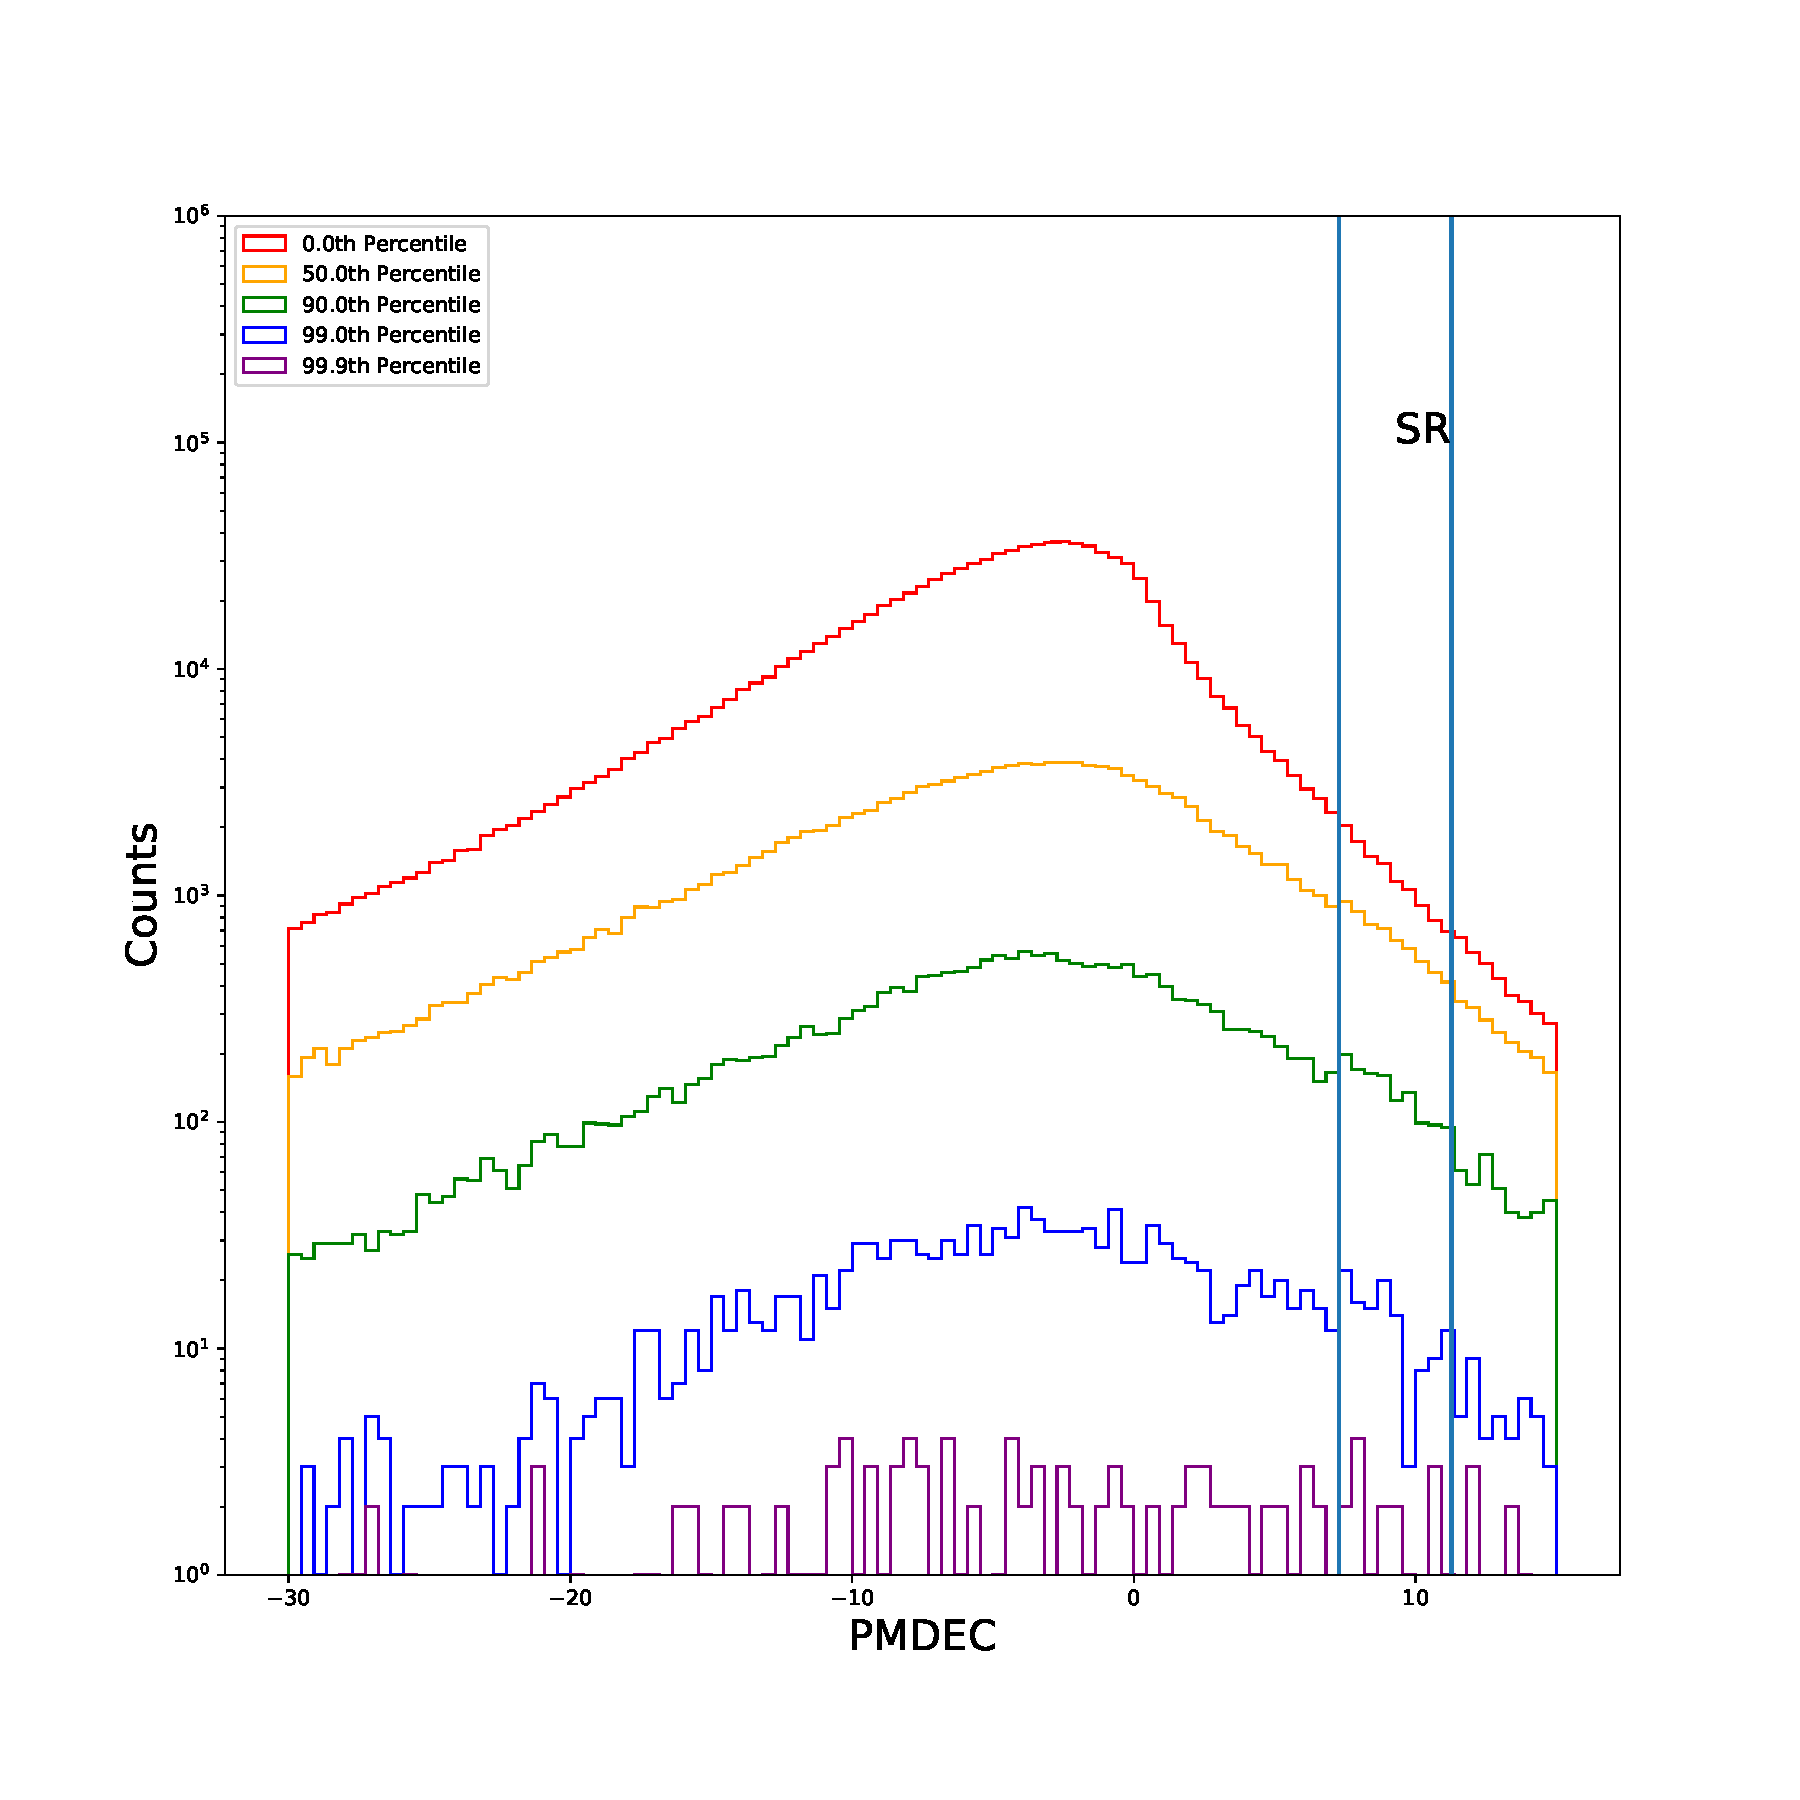
\includegraphics[width=0.5\textwidth]{../figures/scanning_plotsgaiascan_l22_5_b74_4_ra209_6_dec23_3_npy.pdf}
\end{figure}

%===================================================================
\section{Conclusions} \label{sec:conclusions}
%===================================================================


%===================================================================
\section*{\label{sec::acknowledgments}Acknowledgments}
%===================================================================

This work was supported by the Department of Energy, Office of Science under contract number DE-AC02-05CH11231 and many more...

\bibliography{refs,HEPML}
\bibliographystyle{utphys}


\end{document}
